\documentclass[
  captions=tableheading,
  bibliography=totoc, 
  titepage=firstiscover,
]{scrartcl}

\usepackage{blindtext} %neuer input

\usepackage{longtable} % Tabellen über mehrere Seiten

\usepackage[utf8]{inputenc} %neuer input

\usepackage{scrhack}

\usepackage[aux]{rerunfilecheck} %Warnung falls nochmal kompiliert werden muss

\usepackage{fontspec} %Fonteinstellungen

\recalctypearea{}

\usepackage[main=ngerman]{babel} %deutsche Spracheinstellung

\usepackage{ragged2e} %neuer input

\usepackage{amsmath, nccmath}

\usepackage{amssymb} %viele mathe Symbole

\usepackage{mathtools} %Erweiterungen für amsmath


\DeclarePairedDelimiter{\abs}{\lvert}{\rvert}
\DeclarePairedDelimiter{\norm}{\lVert}{\rVert}

\DeclarePairedDelimiter{\bra}{\langle}{\rvert}
\DeclarePairedDelimiter{\ket}{\lvert}{\rangle}

\DeclarePairedDelimiterX{\braket}[2]{\langle}{\rangle}{
#1 \delimsize| #2
}

\NewDocumentCommand \dif {m}
{
\mathinner{\symup{d} #1}
}


\usepackage[
  math-style=ISO,
  bold-style=ISO,
  sans-style=italic,
  nabla=upright,
  partial=upright,
  warnings-off={
    mathtools-colon,
    mathtools-overbracket,
  },
]{unicode-math}

\setmathfont{Latin Modern Math}
\setmathfont{XITS Math}[range={scr, bfscr}]
\setmathfont{XITS Math}[range={cal, bfcal}, StylisticSet=1]


\usepackage[
  locale=DE,
  separate-uncertainty=true,
  per-mode=reciprocal,
  output-decimal-marker={,},
]{siunitx}

\usepackage[autostyle]{csquotes} %richtige Anführungszeichen

\usepackage{xfrac}

\usepackage{float}

\floatplacement{figure}{htbp}

\floatplacement{table}{htbp}

\usepackage[ %floats innerhalb einer section halten
  section,   %floats innerhalb er section halten
  below,     %unterhalb der Section aber auf der selben Seite ist ok
]{placeins}

\usepackage[
  labelfont=bf,
  font=small,
  width=0.9\textwidth,
]{caption}

\usepackage{subcaption} %subfigure, subtable, subref

\usepackage{graphicx}

\usepackage{grffile}

\usepackage{booktabs}

\usepackage{microtype} %Verbesserungen am Schriftbild

\usepackage[
backend=biber,
]{biblatex}

\addbibresource{../lit.bib}

\usepackage[ %Hyperlinks im Dokument
  german,
  unicode,
  pdfusetitle,
  pdfcreator={},
  pdfproducer={},
]{hyperref}

\usepackage{bookmark}

\usepackage[shortcuts]{extdash}

%\usepackage{warpcol}

\usepackage{tikz}

\newcommand*\circled[1]{\tikz[baseline=(char.base)]{
            \node[shape=circle,draw,inner sep=2pt] (char) {#1};}}

\begin{document}
    \title{V602: Röntgenemission und -absorption}
    \author{  
    Paul Störbrock\\
    \texorpdfstring{\href{mailto:paul.stoerbrock@tu-dortmund.de}{paul.stoerbrock@tu-dortmund.de}}{}
    }
    \date{Abgabe: 19.05.2020\vspace{-4ex}}
\maketitle
    
\newpage
\tableofcontents
\newpage

\setcounter{page}{1}

\section{Ziel}

\flushleft{Das\;}\justifying Ziel dieses Versuches ist das Auflösevermögen der $K_{\alpha}$- und $K_{\beta}$-Linie des Kupferröhrenspektrums
zu untersuchen. Außerdem werden anhand der Energien der K-Kanten von den Absorptionsspektren verschiedener Materialien die Abschirmkonstanten bestimmt. 
Mithilfe der Energien und den Abschirmkonstanten lässt sich die Rydbergfrequenz $R$ berechnen. 

\section{Theorie}

\flushleft{Röntgenstrahlung\;}\justifying wird erzeugt, indem Elektronen von einer Glühkathode in einer evakuierten Rühre zu einer
Anode beschleunigt werden. Trifft ein beschleunigtes Elektron auf die Anode, wird das Elektronen abgebremst und verliert Energie. Die Abbremsung
erfolgt im Coulombfeld eines Atomkerns der Anode. Die verlorene Energie wird als Photon (Röntgenquant) abgestrahlt, welches ein kontinuierliches 
Bremsspektrum erzeugt. Das erzeugte Spektrum des emittierten Röntgenquants besitzt die charakteristik des Anodenmaterials. Das Bremsspektrum ist 
kontinuierlich, da das Elektron dessen gesamte kinetische Energie verlieren kann. 

\flushleft{Bei\;}\justifying der Wechselwirkung zwischen Elektron und Anode, wird das Anodenmaterial ionisiert, das heißt, dass ein Elektron der
Anode auf ein höheres Energieniveau gebracht wird. Dies geschieht, indem das Elektron auf eine äußere Schale gestoßen wird. Da eine Leerstelle auf der
inneren Schale entstanden ist, kann ein Elektron von einer äußeren Schale auf die innere zurückfallen, also auf ein niedrigeres Energieniveau.
Demnach ist die Energiedifferenz $h\cdot\nu=E_m - E_n$ \cite{V602} der beiden Schalen $m,n$ die Energie des emittierten Röntgenquants. 
Das charakteristische Spektrum besitzt scharfe Linien, welche als $K_{\alpha}, K_{\beta}, L_{\alpha}, L_{\beta}, M_{\alpha},...$ beschrieben werden. 
Die Buchstaben bezeichnen die Schale, wohingegen $\alpha$ oder $\beta$ die Zielschale des Elektrons bestimmt, welche dessen Energie abgestrahlt 
hat. 

\flushleft{Elektronen\;}\justifying auf einer höheren Schale erfahren eine geringere Anziehungskraft des Atomkerns, da Elektronen auf einer tieferen
Schale einen Teil der Kernladung abschirmen. Die Bindungsenergie zwischen einem Elektron auf der $n$-ten Schale kann dementsprechend mit der 
Formel \cite{V602}
\begin{align}
    E_n = -R_{\infty}\cdot z_{eff}^2 \cdot \frac{1}{n^2} \label{eq:1}
\end{align}
\flushleft{dargestellt\;}\justifying werden. Hierbei ist die Rydbergenergie $R_{\infty}=\SI{13.6}{\electronvolt}$ und 
\begin{align}
    z_{eff}=z-\sigma \label{eq:2}
\end{align}
\flushleft{die\;}\justifying effetive Kernladung, wobei z die Ordnungszahl des Elements und $\sigma$ die Abschirmkonstante darstellt. 
Da neben der Coulomb Anziehung die Elektronen selbst durch den eigenen Spin und dem Bahndrehimpuls miteinander wechselwirken, sind die
charakteristischen Linien des Spektrums nicht scharf definiert. Die einzelnen Linien sind in eng beieinander liegenden Linien unterteilt. Diese 
Unterteilung heißt Feinstruktur, welche mit diesem Versuch hingegen nicht aufgelöst werden kann. 

\flushleft{Die\;}\justifying Absorption eines Materials ist energiebedingt und hängt von der Bindungsenergie ab. Wird die Bindungsenergie 
überschritten, wird das Elektron aus der jeweiligen Schale gelöst. Entweder wird das Elektron auf eine energetisch höhere Schale gestoßen 
(Compton-Effekt), oder es wird ganz aus der Umlaufbahn des Atoms geworfen (Photoeffekt). Das Absorptionsspektrum fällt mit zunehmender Energie ab und erzeugt
Peaks, wenn die Bindungsenergie überschritten wird. Diese Peaks im Graphen werden als Absorptionskanten bezeichnet und als $K-, L-, M-,...$ Kante definiert. 
Die hier relevante Kante ist die $K-$Kante. Da das Absorptionsspektrum analog zum Emissionsspektrum nicht scharf definiert ist, muss die Bindungsenergie
eines Elektrons mit der Sommerfeldschen Feinstrukturformel \cite{V602} 
\begin{align}
    E_{n,j} &= -R_{infty} \left( z_{eff,1}^2 \cdot \frac{1}{n^2} + \alpha^2 z_{eff,2}^4 \cdot \frac{1}{n^3} \left( \frac{1}{j+\frac{1}{2}} - \frac{3}{4n} \right) \right) \label{eq:3}
\end{align}
\flushleft{bestimmt\;}\justifying werden. $R_{\infty}$ ist hier wieder die Rydbergenergie, $z_{eff}$ die Kernladungszahl, $\alpha$ die 
Sommerfeldsche Feinstrukturkonstante, $n$ die Hauptquantenzahl und $j$ der Gesamtdrehimpuls des jeweiligen Elektrons. Wird $z_{eff}=z-\sigma$
eingesetzt, lässt sich die Sommerfeldsche Feinstrukturformel zu der Abschirmkonstante $\sigma_{K,abs}$ umstellen. Daraus folgt: \cite{V602}
\begin{align}
    \sigma_{K,abs} &= z - \sqrt{\frac{E_K}{R_{\infty}} - \frac{\alpha^2 z^4}{4}} \label{eq:4}
\end{align}
\flushleft{Die\;}\justifying Rydbergenergie $R_{\infty}= R\cdot h$ ist definiert durch die Rydbergfrequenz $R$ und dem plankschen Wirkungsquantum $h$.
Das Moseley'sche Gesetzt erlaubt es die Energie $E_{K_{\alpha}}$ durch eine Proportionalität zu $z_{eff}^2$ als 
\begin{align}
    E_{K_{\alpha}} &= Rh \left( z-\sigma \right)^2 \label{eq:Mosel}
\end{align}
\flushleft{zu\;}\justifying approximieren. Durch Umstellen dieser Gleichung lässt sich die Geradengleichung
\begin{align}
    \sqrt{E_{K_{\alpha}}} &= \sqrt{Rh}\cdot z_{eff}^2 \label{eq:RyGl}
\end{align}
\flushleft{bestimmen.\;}\justifying Dabei ist $\sqrt{Rh}$ die Steigung $m$, woraus sich die Rydbergfrequenz
\begin{align}
 R &= \frac{m^2}{h} \label{eq:Ryf}
 \end{align}
\flushleft{ergibt.}
\newpage
\flushleft{Die\;}\justifying Energie des emittierten Photons 
\begin{align}
    E=\frac{hc}{\lambda e} \label{eq:5}
    \intertext{lässt sich mithilfe der Bragg'schen Bedingung
    }
    2d\sin(\theta) &= n\lambda \label{eq:6}
\end{align}
\flushleft{bestimmen.\;}\justifying Die Bragg'sche Reflexion bezeichnet die Beugung der emittierten Röntgenstrahlung an einem Lithiumfluorid-Kristall (LiF-Kristall).
Dabei ist $d_{LiF}=\SI{201.4}{\pico\meter}$ \cite{V602} die Gitterkonstante des LiF-Kristalls, $\lambda$ die Wellenlänge der Strahlung, $\theta$
der Glanzwinkel und $n$ die Ordnungszahl des Materials. Das atomare Gitter des LiF-Kristalls beugt die Photonen und erzeugt im Glanzwinkel konstruktive 
Interferenz. 

\flushleft{Da\;}\justifying das Emissionsspektrum aufgrund der Sommerfeldschen Feinstruktur nicht eindeutig ist, sondern die Sprünge bzw. Peaks in 
einem Intervall liegen, wird für die Breite der Linien das Auflösevermögen 
\begin{align}
    A = \frac{E_K}{\Delta E_{FWHM}} \label{eq:7}
\end{align}
bestimmt werden. $E_K$ ist hierbei die jeweilige Kantenenergie und $\Delta E_{FWHM}$ ist die jeweilige Energie der Halbwertsbreite (HWB). Die HWB
beschreibt die Länge des Intervalls, in welcher sich die betrachtete Kante befindet. Im Falle von Kupfer werden die $K_{\alpha}$- und die
$K_{\beta}$-Linie betrachtet, welche in dem jeweiligen Intervall der $HWB_{K_{\alpha}}$ und $HWB_{K_{\beta}}$ liegen. Die halbe Amplitude der $K_{\alpha}$- 
bzw. $K_{\beta}$-Linie beschreibt Anfang und Ende der HWB. Die DiffAus der Differenz der Grenzen der HWB lässt sich die Energie der jeweiligen HWB
bestimmen, welche zum Auflösevermögen der Linie führt.

\section{Versuchsaufbau und -durchführung}

\flushleft{Materialien:\;}\justifying \textit{Eine Kupfer-Röntgenröhre, ein LiF-Kristall, ein Geiger-Müller Zählrohr, ein Röntgengerät, ein 
Bromabsorber, ein Galliumabsorber, ein Rubidiumabsorber, ein Strontiumabsorber, ein Zinkabsorber und ein Zirkoniumabsorber.}

\newpage
\flushleft{Das\;}\justifying Röntgengerät wird wie folgt aufgebaut:
\begin{figure}[H]
    \centering
    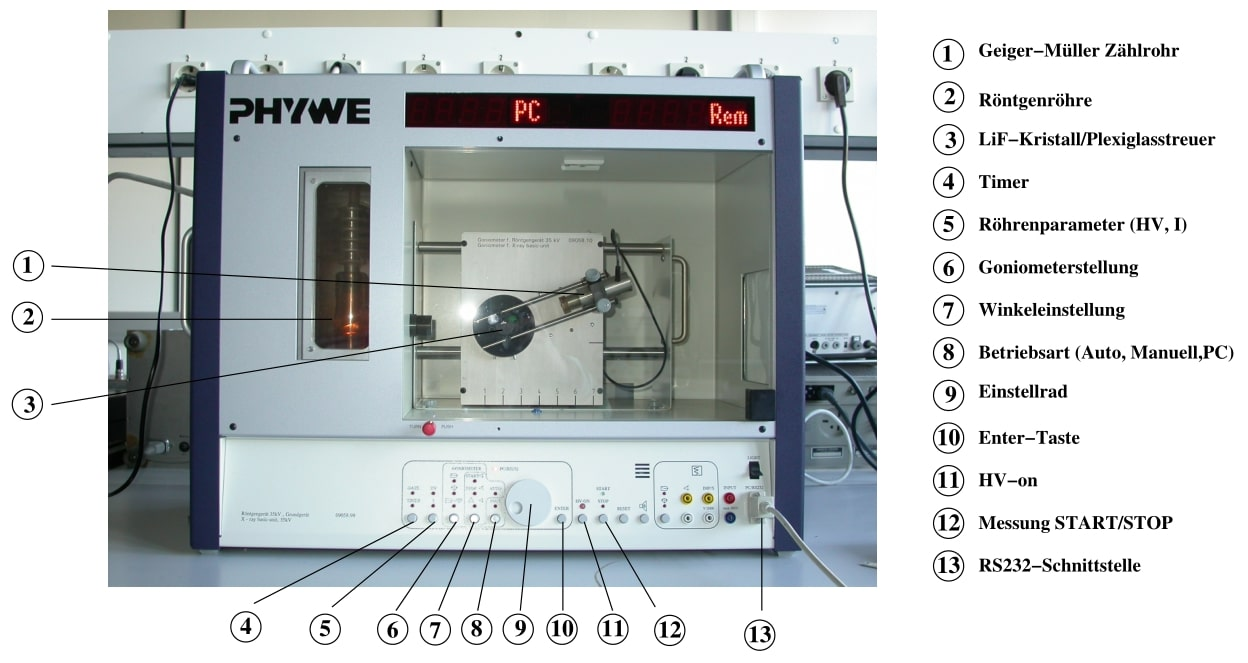
\includegraphics[width=\textwidth]{./images/Röntgenröhre.jpg}
    \caption{Aufbau der Röntgenröhre \cite{V602}}
    \label{fig:1}
\end{figure}
\flushleft{Zu\;}\justifying Beginn wird die Bragg Bedingung überprüft. Dazu wird der LiF-Kristall auf einen festen Winkel von $\theta=\SI{14}{\degree}$ gestellt und der
Winkelbereich des Geiger-Müller Zählrohrs variiert. Der Winkelbereich liegt zwischen $\SI{26}{\degree}\leq\alpha\leq\SI{30}{\degree}$ und wird in
$\SI{0.1}{\degree}$-Schritten bei einer Integrationszeit von $\Delta t=\SI{5}{\second}$ pro Winkel durchlaufen. 

\flushleft{Um\;}\justifying das Emissionsspektrum der Kupferröhre zu bestimmen wird diesmal das Geiger-Müller Zählrohr um den doppelten Winkel
zum LiF-Kristall variiert. Der Winkelbereich des LiF-Kristalls liegt hier zwischen $\SI{8}{\degree}\leq\alpha\leq\SI{25}{\degree}$ und wird ebenfalls in 
$\SI{0.1}{\degree}$-Schritten bei einer Integrationszeit von $\Delta t=\SI{5}{\second}$ pro Winkel durchlaufen.

\flushleft{Für\;}\justifying das Absorptionsspektrum der anderen Materialien wird der entsprechende Absorber angebracht. Hier wird der Winkelbereich
ebenfalls in $\SI{0.1}{\degree}$-Schritten durchlaufen, jedoch bei einer Integrationszeit von je $\Delta t=\SI{20}{\second}$ pro Winkel.
Die Winkelintervalle lauten wie folgt:\\
\begin{align*}
    \SI{12.8}{\degree}  &\leq\theta_{\text{Brom}}\leq\SI{14.3}{\degree},\\ 
    \SI{17}{\degree}    &\leq\theta_{\text{Gallium}}\leq\SI{19}{\degree},\\
    \SI{11.2}{\degree}  &\leq\theta_{\text{Rubidium}}\leq\SI{12.5}{\degree},\\
    \SI{10.5}{\degree}  &\leq\theta_{\text{Strontium}}\leq\SI{12}{\degree},\\
    \SI{18}{\degree}    &\leq\theta_{\text{Zink}}\leq\SI{19.5}{\degree}\;\text{und}\\
    \SI{9.5}{\degree}   &\leq\theta_{\text{Zirkonium}}\leq\SI{11}{\degree}.
\end{align*}


\section{Auswertung}

\subsection{Bragg'sche Bedingung}

    \flushleft{Um\;}\justifying die Bragg'sche Bedingung zu überprüfen, wird die Intesität der Röntgenstrahlung gegen den Winkel $\theta$ des
    Geiger-Müller Zählrohrs graphisch aufgetragen. Dazu werden die Werte aus die Tabelle \ref{tab:2} und die Pythonbibliothek matplotlib 
    \cite{matplotlib} verwendet. Alle folgendenen Graphen werden mit matplotlib erstellt. Der Graph der Bragg'schen Bedingung sieht aus wie
    folgt:

    \begin{figure}[H]
        \centering
        \includegraphics[width=\textwidth]{build/plotBragg.pdf}
        \caption{Hier wird die Impulsrate gegen den Variationswinkel $\theta$ des Geiger-Müller Zählrohrs graphisch aufgetragen. 
        Außerdem ist die Maximale Impulsrate, sowie die Ausgleichskurve der Gaußverteilung eingezeichnet.}
        \label{fig:2}
    \end{figure}

    \flushleft{Da\;}\justifying es sich bei der Werteverteilung im Graph \ref{fig:2} um eine Gaußverteilung handelt, wird die Ausgleichskurve 
    mit dem Pythonbefehl curve\_fit \cite{matplotlib} unter Verwendung der Formel der Gaußkurve
    \begin{align}
        \theta &= a\cdot \exp\left(-\left(\frac{x-b}{c}\right)^2\right)\cdot d \label{eq:8}
    \end{align}
    \flushleft{erstellt.\;}\justifying Die dazugehörigen Parameter lauten:
    \begin{subequations}\label{eq:9}
        \begin{align*}
            a &= \text{\input{a.tex}}\\
            b &= \text{\input{b.tex}}\\
            c &= \text{\input{c.tex}}\\
            d &= \text{\input{d.tex}}
        \end{align*}
    \end{subequations}
    \flushleft{Das\;}\justifying in Graph \ref{fig:2} eingezeichnete Maximum liegt bei 
    \begin{subequations}\label{eq:10}
    \begin{align}
        \theta &= \text{\input{xmax_bragg.tex}} \label{eq:10a}\\
        N &= \text{\input{ymax_bragg.tex}}. \label{eq:10b}
    \end{align}
    \end{subequations}

\subsection{Auflösevermögen der K-Linien des Kupferemissionsspektrums}

    \flushleft{Für\;}\justifying das Emissionsspektrum von Kupfer werden die Werte aus Tabelle \ref{tab:1} wie folgt gegeneinander aufgetragen:

    \begin{figure}[H]
        \centering
        \includegraphics[width=\textwidth]{build/plotCu.pdf}
        \caption{Hier wird das Emissionsspektrum der Kupferröhre anhand der Impulsrate und des Variationswinkels $\theta$ dargestellt. Die farbig-
        gepunkteten Linien bezeichnen die $K_{\alpha}$- bzw. $K_{\beta}$-Linie. Die grauen Linien sind die Schranken der Halbwertsbreite
        der jeweiligen Linie.}
        \label{fig:3}
    \end{figure}

    \flushleft{Anhand\;}\justifying des Graphen lassen sich die $K_{\alpha}$- und die $K_{\beta}$-Linie ablesen. Diese liegen bei einem
    Winkel $\theta$ von:
    \begin{subequations}\label{eq:11}
    \begin{align}
        \theta_{K_{\alpha}} &= \text{\input{xmax_cu.tex}} \label{eq:11a}\\
        \theta_{K_{\beta}} &= \text{\input{xlmax_cu.tex}} \label{eq:11b}
    \end{align}
    \end{subequations}
    \flushleft{Durch\;}\justifying Umstellen der Formel \eqref{eq:6} nach $\lambda = 2d\cdot\sin(\theta)$ für $n=1$ lassen sich die Wellenlängen 
    der beiden Linien bestimmen: 
    \begin{subequations}\label{eq:12}
    \begin{align}
        \lambda_{K_{\alpha}} &= \text{\input{L_cu_a.tex}} \label{eq:12a}\\
        \lambda_{K_{\beta}} &= \text{\input{L_cu_b.tex}} \label{eq:12b}
    \end{align}
    \end{subequations}
    \flushleft{Es\;}\justifying ist zu beachten, dass hier alle Winkel $\theta$ mit einem Fehler $\Delta \theta$ von \SI{0.1}{\degree} behaftet ist.
    
    \flushleft{Dieser\;}\justifying Fehler wird mit der gaußschen Fehlerfortpflanzung berechnet:
    \begin{align} 
    \Delta E &= \frac{hc \cos(\theta)}{2d\sin^2(\theta)} \cdot \sigma_{\theta}
    \end{align}
    Hier wird der Fehler mithilfe eines ufloats \cite{uncertainties} an Python übergeben. 
    Mithilfe der Formel \eqref{eq:5} lassen sich die jeweiligen Energien für die $K_{\alpha}$- und $K_{\beta}$-Linie
    berechnen. Diese lauten:
    \begin{subequations}\label{eq:13}
    \begin{align}
        E_{K_{\alpha}} &= \text{\input{E_cu_a.tex}} \label{eq:13a}\\
        E_{K_{\beta}} &= \text{\input{E_cu_b.tex}} \label{eq:13b}
    \end{align}
    \end{subequations}
    \flushleft{Da\;}\justifying die Linien nicht eindeutig definiert sind, wird das Auflösevermögen der beiden Kanten bestimmt. Dazu wird die 
    Halbwertsbreite der einzelnen Linien benötigt. Die Halbwertsbreiten lassen sich dem Graphen \ref{fig:3} entnehmen. Mithilfe der 
    Halbwertsbreiten lässt sich $\Delta E_{FWHM}$ bestimmen, wofür die Wellenlänge der Kanten der jeweiligen Halbwertsbreite benötigt wird. 
    Die Wellenlängen der Halbwertsbreiten lauten:
    \begin{subequations}\label{eq:14}
    \begin{align}
        \lambda_{K_{\alpha},links} &= \text{\input{L_HWB_cu_a_links.tex}} \qquad \text{für}\;\theta = 22.35 \label{eq:14a}\\
        \lambda_{K_{\alpha},rechts} &= \text{\input{L_HWB_cu_a_rechts.tex}} \qquad \text{für}\;\theta = 22.85 \label{eq:14b}\\
        \lambda_{K_{\beta},links} &= \text{\input{L_HWB_cu_b_links.tex}} \qquad \text{für}\;\theta = 20.05 \label{eq:14c}\\
        \lambda_{K_{\beta},rechts} &= \text{\input{L_HWB_cu_b_rechts.tex}} \qquad \text{für}\;\theta = 22.55 \label{eq:14d}
    \end{align}
    \end{subequations}
    \flushleft{Die\;}\justifying daraus nach Formel \eqref{eq:5} resultierenden Energien lauten:
    \begin{subequations}\label{eq:15}
    \begin{align}
        E_{K_{\alpha},links} &= \text{\input{E_HWB_cu_a_links.tex}} \label{eq:15a}\\
        E_{K_{\alpha},rechts} &= \text{\input{E_HWB_cu_a_rechts.tex}} \label{eq:15b}\\
        E_{K_{\beta},links} &= \text{\input{E_HWB_cu_b_links.tex}} \label{eq:15c}\\
        E_{K_{\beta},rechts} &= \text{\input{E_HWB_cu_b_rechts.tex}} \label{eq:15d}
    \end{align}
    \end{subequations}
    \flushleft{Für\;}\justifying $\Delta E_{FWHM}$ wird der Absolutbetrag der Differenz der jeweiligen $E_{K_{\alpha,\beta},links,rechts}$ benötigt.
    Also ergibt sich für $\Delta E_{FWHM}$:
    \begin{subequations}\label{eq:16}
    \begin{align}
        \Delta E_{FWHM, \alpha} &= \vert E_{K_{\alpha},rechts}-E_{K_{\alpha},links} \vert = \text{\input{E_HWB_cu_a.tex}} \label{eq:16a}\\
        \Delta E_{FWHM, \beta} &= \vert E_{K_{\beta},rechts}-E_{K_{\beta},links} \vert = \text{\input{E_HWB_cu_b.tex}} \label{eq:16b}
    \end{align}
    \end{subequations}
    \flushleft{Werden\;}\justifying die Energien $E_{K_{\alpha, \beta}}$ der $K_{\alpha,\beta}$-Linie und die Energien der HWB 
    $\Delta E_{FWHM, \alpha, \beta}$ in Formel \eqref{eq:7} eingesetzt, ergibt sich für die jeweiligen Auflösevermögen:
    \begin{subequations}\label{eq:17}
    \begin{align}
        A_{K_{\alpha}} &= \text{\input{A_cu_a.tex}} \label{eq:17a}\\
        A_{K_{\beta}} &= \text{\input{A_cu_b.tex}} \label{eq:17b}
    \end{align}
    \end{subequations}
    \flushleft{Anschließend\;}\justifying werden die Abschirmkonstanten $\sigma_{1,2,3}$ für Kupfer bestimmt. Dazu wird die Formel \eqref{eq:3}
    verwendet, wobei der Drehimpulsbeitrag $\left( \frac{1}{j+\frac{1}{2}} \right)$ vernachlässigt wird. Daraus folgen die Abschätzungen:
    \begin{subequations}\label{eq:18}
    \begin{align}
        E_{K,abs} &= R_{\infty} (z-\sigma_1)^2 \label{eq:18a}\\
        E_{K,\alpha} &= R_{\infty} \left( \frac{1}{n} \right)^2 (z-\sigma_1)^2 - R_{\infty} \left( \frac{1}{m} \right)^2 (z-\sigma_2)^2 \label{eq:18b}\\
        E_{K,\beta} &= R_{\infty} \left( \frac{1}{n} \right)^2 (z-\sigma_1)^2 - R_{\infty} \left( \frac{1}{l} \right)^2 (z-\sigma_3)^2 \label{eq:18c}
    \end{align}
    \end{subequations}
    \flushleft{Hier\;}\justifying werden $n=1$, $m=2$ und $l=3$ gesetzt. Die Ornungszahl $z$ von Kupfer ist 29. Da sich $\sigma_1$ hier nicht ermitteln lässt, 
    wird der Literaturwert für die Absorptionsenergie $E_{K,abs}= \text{\input{E_Kedge_cu.tex}}$ eingesetzt. Die daraus folgende 
    Abschirmkonstante lautet:
    \begin{align}
        \sigma_1 &= \text{\input{sigma1_cu.tex}} \label{eq:19}
    \end{align}
    \flushleft{Wird\;}\justifying $z_{eff,1}^2=\sfrac{E_{K,abs}}{R_{\infty}}$ in Gleichungen \eqref{eq:18b} und \eqref{eq:18c} eingesetzt,
    folgt durch jeweiliges Umformen:
    \begin{subequations}\label{eq:20}
    \begin{align}
        \sigma_2 &= z-\sqrt{4\cdot\frac{E_{K,abs}-E_{K_{\alpha}}}{R_{\infty}}} = \text{\input{sigma2_cu.tex}} \label{eq:20a}\\
        \sigma_3 &= z-\sqrt{9\cdot\frac{E_{K,abs}-E_{K_{\beta}}}{R_{\infty}}} = \text{\input{sigma3_cu.tex}} \label{eq:20b}
        \intertext{\flushleft{Wobei\;}\justifying sich die Fehlerfortpflanzung der Energien $\delta E_{K_{\alpha,\beta}}$ wie folgt ergibt: 
        }
        \Delta E_{K_{\alpha,\beta}} &= \frac{m,l}{2}\sqrt{ \frac{\sigma_{E_{\alpha,\beta}}^2}{(E_{K,abs}-E_{K_{\alpha,\beta}})E_{\infty}}}
    \end{align}
    \end{subequations}

\newpage
\subsection{Absorptionsenergie und Abschirmkonstante von Brom}

    \flushleft{Der\;}\justifying folgende Graph \ref{fig:4} gibt das Absorptionsspektrum von Brom mithilfe der Messwerte aus Tabelle \ref{tab:3} 
    wieder. 

    \begin{figure}[H]
        \centering
        \includegraphics[width=\textwidth]{build/plotBr.pdf}
        \caption{Absorptionsspektrum des Bromabsorbers}
        \label{fig:4}
    \end{figure}

    \flushleft{Um\;}\justifying die Absorptionsenergie $E_{K,Br}$ zu bestimmen, wird die Mitte der K-Kante bestimmt. Das erfolgt mit der
    Formel \cite{V602}
    \begin{subequations}\label{eq:21}
    \begin{align}
        I_K &= I_K^{min} + \frac{I_K^{max}-I_K^{min}}{2}. \label{eq:21a}
        \intertext{Die Extrema der Intesität liegen hier bei:
        }
        I_{max} &= \text{\input{I_max_br.tex}} \label{eq:21b}\\
        I_{min} &= \text{\input{I_min_br.tex}} \label{eq:21c}
        \intertext{Daraus folgt die mittlere Intensität
        }
        I_K &= \text{\input{I_K_br.tex}} \label{eq:21d}
        \intertext{womit sich der Winkel $\theta_K$ aus dem Graphen ablesen lässt:
        }
        \theta_K &= \text{\input{theta_K_br.tex}} \label{eq:21e}
        \intertext{Mithilfe des Winkels $\theta_K$ lassen sich analog zum Emissionsspektrum von Kupfer die Wellenlänge $\lambda_K$ mit Formel
        \eqref{eq:6} und Energie $E_K$ mit Formel \eqref{eq:5} berechnen:
        }
        \lambda_K &= \text{\input{L_K_br.tex}} \label{eq:21f}\
        \intertext{
            Hier ist die Fehlerfortpflanzung analog zum Kupferemissionsspektrum wieder:
        }
        \Delta E &= \frac{hc \cos(\theta)}{2d\sin^2(\theta)} \cdot \sigma_{\theta}
        \intertext{
            Woraus sich für die Energie ergibt:
        }
        E_{K,Br} &= \text{\input{E_K_br.tex}} \label{eq:21g}
        \intertext{Abschließend wird die Abschirmkonstante $\sigma_{Br}$ mithilfe von Formel \eqref{eq:4} bestimmt, wobei die Ornungszahl von Brom
        $z=35$ \cite{NIST} ist:
        }
        \sigma_{Br} &= \text{\input{sigma_br.tex}} \label{eq:21h}
        \intertext{
            Für die Fehlerfortpflanzung ergibt sich analog zum Kupferemissionsspektrum, aber mit Formel \eqref{eq:4}:
        }
        \Delta\sigma &= \frac{1}{2} \sqrt{ \frac{\sigma_{E_K}^2}{E_{\infty}^2 \left( \frac{E_K}{E_{\infty}}-\frac{\alpha^2 z^4}{4} \right)}}
        \intertext{
            Hierbei wird die Ordnungszahl $z$ und die Energie $E_K$ dem jeweiligen Absorbermaterial angepasst.
        }
    \end{align}
    \end{subequations}

    \textit{\flushleft{Mit\;}\justifying den folgenden Absorbern wird analog zum Bromabsorber verfahren, weshalb im Folgenden nur noch die 
    Ergebnisse angegeben werden.}

\subsection{Absorptionsenergie und Abschirmkonstante von Gallium}

    \flushleft{Der\;}\justifying folgende Graph \ref{fig:4} gibt das Absorptionsspektrum von Gallium mithilfe der Messwerte aus Tabelle \ref{tab:4} 
    wieder.

    \begin{figure}[H]
        \centering
        \includegraphics[width=\textwidth]{build/plotGa.pdf}
        \caption{Absorptionsspektrum des Galliumabsorbers}
        \label{fig:5}
    \end{figure}

    \flushleft{Ergebnisse\;}\justifying für den Galliumabsorber:
    \begin{subequations}\label{eq:22}
    \begin{align}
        I_{max} &= \text{\input{I_max_ga.tex}} \label{eq:22a}\\
        I_{min} &= \text{\input{I_min_ga.tex}} \label{eq:22b}\\
        \Rightarrow I_K &= \text{\input{I_K_ga.tex}} \label{eq:22c}\\
        \Rightarrow \theta_K &= \text{\input{theta_K_ga.tex}} \label{eq:22d}\\
        \stackrel{\eqref{eq:6}}{\Rightarrow} \lambda_K &= \text{\input{L_K_ga.tex}} \label{eq:22e}\\
        \stackrel{\eqref{eq:5}}{\Rightarrow} E_{K,Ga} &= \text{\input{E_K_ga.tex}} \label{eq:22f}\\
        \Rightarrow \sigma_{Ga} &= \text{\input{sigma_ga.tex}} \qquad \text{mit}\; z=31\; \text{\cite{NIST}} \label{eq:22g}
    \end{align}
    \end{subequations}

\subsection{Absorptionsenergie und Abschirmkonstante von Rubidium}

    \flushleft{Der\;}\justifying folgende Graph \ref{fig:4} gibt das Absorptionsspektrum von Rubidium mithilfe der Messwerte aus Tabelle \ref{tab:5a} 
    wieder.

    \begin{figure}[H]
        \centering
        \includegraphics[width=\textwidth]{build/plotRb.pdf}
        \caption{Absorptionsspektrum des Rubidiumabsorbers}
        \label{fig:6}
    \end{figure}

    \flushleft{Ergebnisse\;}\justifying für den Rubidiumabsorber:
    \begin{subequations}\label{eq:23}
    \begin{align}
        I_{max} &= \text{\input{I_max_rb.tex}} \label{eq:23a}\\
        I_{min} &= \text{\input{I_min_rb.tex}} \label{eq:23b}\\
        \Rightarrow I_K &= \text{\input{I_K_rb.tex}} \label{eq:23c}\\
        \Rightarrow \theta_K &= \text{\input{theta_K_rb.tex}} \label{eq:23d}\\
        \stackrel{\eqref{eq:6}}{\Rightarrow} \lambda_K &= \text{\input{L_K_rb.tex}} \label{eq:23e}\\
        \stackrel{\eqref{eq:5}}{\Rightarrow} E_{K,Rb} &= \text{\input{E_K_rb.tex}} \label{eq:23f}\\
        \Rightarrow \sigma_{Rb} &= \text{\input{sigma_rb.tex}} \text{mit}\; z=37\; \text{\cite{NIST}} \label{eq:23g}
    \end{align}
    \end{subequations}

\subsection{Absorptionsenergie und Abschirmkonstante von Strontium}

    \flushleft{Der\;}\justifying folgende Graph \ref{fig:4} gibt das Absorptionsspektrum von Strontium mithilfe der Messwerte aus Tabelle \ref{tab:5b} 
    wieder.

    \begin{figure}[H]
        \centering
        \includegraphics[width=\textwidth]{build/plotSr.pdf}
        \caption{Absorptionsspektrum des Strontiumabsorbers}
        \label{fig:7}
    \end{figure}

    \flushleft{Ergebnisse\;}\justifying für den Strontiumabsorber:
    \begin{subequations}\label{eq:24}
    \begin{align}
        I_{max} &= \text{\input{I_max_sr.tex}} \label{eq:24a}\\
        I_{min} &= \text{\input{I_min_sr.tex}} \label{eq:24b}\\
        \Rightarrow I_K &= \text{\input{I_K_sr.tex}} \label{eq:24c}\\
        \Rightarrow \theta_K &= \text{\input{theta_K_sr.tex}} \label{eq:24d}\\
        \stackrel{\eqref{eq:6}}{\Rightarrow} \lambda_K &= \text{\input{L_K_sr.tex}} \label{eq:24e}\\
        \stackrel{\eqref{eq:5}}{\Rightarrow} E_{K,Sr} &= \text{\input{E_K_sr.tex}} \label{eq:24f}\\
        \Rightarrow \sigma_{Sr} &= \text{\input{sigma_sr.tex}} \text{mit}\; z=38\; \text{\cite{NIST}} \label{eq:24g}
    \end{align}
    \end{subequations}

\subsection{Absorptionsenergie und Abschirmkonstante von Zink}

    \flushleft{Der\;}\justifying folgende Graph \ref{fig:4} gibt das Absorptionsspektrum von Zink mithilfe der Messwerte aus Tabelle \ref{tab:5c} 
    wieder.

    \begin{figure}[H]
        \centering
        \includegraphics[width=\textwidth]{build/plotZn.pdf}
        \caption{Absorptionsspektrum des Zinkabsorbers}
        \label{fig:8}
    \end{figure}

    \flushleft{Ergebnisse\;}\justifying für den Zinkabsorber:
    \begin{subequations}\label{eq:25}
    \begin{align}
        I_{max} &= \text{\input{I_max_zn.tex}} \label{eq:25a}\\
        I_{min} &= \text{\input{I_min_zn.tex}} \label{eq:25b}\\
        \Rightarrow I_K &= \text{\input{I_K_zn.tex}} \label{eq:25c}\\
        \Rightarrow \theta_K &= \text{\input{theta_K_zn.tex}} \label{eq:25d}\\
        \stackrel{\eqref{eq:6}}{\Rightarrow} \lambda_K &= \text{\input{L_K_zn.tex}} \label{eq:25e}\\
        \stackrel{\eqref{eq:5}}{\Rightarrow} E_{K,Zn}K &= \text{\input{E_K_zn.tex}} \label{eq:25f}\\
        \Rightarrow \sigma_{Zn} &= \text{\input{sigma_zn.tex}} \text{mit}\; z=30\; \text{\cite{NIST}} \label{eq:25g}
    \end{align}
    \end{subequations}

\subsection{Absorptionsenergie und Abschirmkonstante von Zirkonium}

    \flushleft{Der\;}\justifying folgende Graph \ref{fig:4} gibt das Absorptionsspektrum von Zirkonium mithilfe der Messwerte aus Tabelle \ref{tab:5d} 
    wieder.

    \begin{figure}[H]
        \centering
        \includegraphics[width=\textwidth]{build/plotZr.pdf}
        \caption{Absorptionsspektrum des Zirkoniumabsorbers}
        \label{fig:9}
    \end{figure}

    \flushleft{Ergebnisse\;}\justifying für den Zirkoniumabsorber:
    \begin{subequations}\label{eq:26}
    \begin{align}
        I_{max} &= \text{\input{I_max_zr.tex}} \label{eq:26a}\\
        I_{min} &= \text{\input{I_min_zr.tex}} \label{eq:26b}\\
        \Rightarrow I_K &= \text{\input{I_K_zr.tex}} \label{eq:26c}\\
        \Rightarrow \theta_K &= \text{\input{theta_K_zr.tex}} \label{eq:26d}\\
        \stackrel{\eqref{eq:6}}{\Rightarrow} \lambda_K &= \text{\input{L_K_zr.tex}} \label{eq:26e}\\
        \stackrel{\eqref{eq:5}}{\Rightarrow} E_{K,Zr} &= \text{\input{E_K_zr.tex}} \label{eq:26f}\\
        \Rightarrow \sigma_{Zr} &= \text{\input{sigma_zr.tex}} \text{mit}\; z=40\; \text{\cite{NIST}} \label{eq:26g}
    \end{align}
    \end{subequations}

\subsection{Rydbergfrequenz}

    \flushleft{Um\;} die Rydbergfrequenz bestimmen zu können, werden die zuvor bestimmten Energien $E_K$ und Abschirmkonstanten $sigma_K$ der
    Absorber in dem folgenden $\sqrt{E_K}-Z$ Diagramm aufgetragen. Dazu wird die Geradengleichung \eqref{eq:RyGl} verwendet. 
    Die Ausgleichsgerade wird mit dem numpy Befehl polyfit \cite{numpy} und den Parametern 
    \begin{subequations}\label{27}
    \begin{align}
        m &= \text{\input{m_ry.tex}}\label{eq:27a}\\
        b &= \text{\input{b_ry.tex}}\label{eq:27b}
    \end{align}
    \end{subequations}
    \flushleft{erstellt.\;}\justifying
    
    \begin{figure}[H]
        \centering
        \includegraphics[width=\textwidth]{build/plotE_K.pdf}
        \caption{Lineare Regression der Rydbergfrequenz}
        \label{fig:10}
    \end{figure}

    \flushleft{Da\;}\justifying hier die Steigung $m$ die Wurzel der Rydbergenergie $\sqrt{R \cdot h}$ darstellt, ist $m^2$ die Rydbergfrequenz $R$
    mal dem plankschen Wirkungsquantum $h$:
    \begin{subequations}\label{28}
    \begin{align}
        m^2 &= R\cdot h = \text{\input{Rydb_const.tex}}\label{eq:28a}
        \intertext{Die Rydbergfrequenz lässt sich also mit $R_f = \frac{R_{\infty} e}{h}$ bestimmen, wobei $e$ die Elementarladung darstellt. 
        Folglich ist die Rydbergfrequenz
        }
        R_f &= \text{\input{Rydb_f.tex}}.\label{eq:28b}
    \end{align}
    \end{subequations}

\newpage
\section{Diskussion}

    \flushleft{Die\;}\justifying Bragg'sche Bedingung behandelt den Glanzwinkel $\theta$, wo konstruktive Interferenz herrscht. Dieser liegt im
    Graphen \ref{fig:2} beim Maximum $\theta = \text{\input{xmax_bragg.tex}}$. Der theoretische Wert ist hier $\theta=\text{\input{theta_bragg_lit.tex}}$,
    was sich geometrisch begründen lässt, da der Einfallswinkel geleich dem Ausfallswinkel sein muss. Der relative Fehler beträgt demnach:
    \begin{align}
        \frac{\theta-\theta_{Lit.}}{\theta_{Lit.}} &= \text{\input{theta_bragg_err.tex}.}\label{eq:29}
    \end{align}
    \flushleft{Der\;}\justifying kleine relative Fehler gibt die Genauigkeit des Messgeräts und die Beschaffenheit des LiF-Kristalls wieder.
    Der Fehler kann auf die Verunreinigungen der Oberfläche des LiF-Kristalls und dem Sauerstoff zwischen Kupferröhre und Geiger-Müller
    Zählrohr zurückgeführt werden. Da die Bragg'sche Bedingung Auskunft über die Genauigkeit der Emissionsspektren, bzw. der Absorptionsspektren
    gibt, indem es die Lage der konstruktiven Interferenz anahnd einer Gaußkurve beschreibt, kann eine Abweichung vom theoretischen Glanzwinkels
    von \SI{1}{\degree} oder \SI{3}{\degree} die Form der Spektren verändern. Die Gaußform der Kurve diktiert, dass die Intensität in beiden 
    Richtungen vom Maximum schnell abfällt, also würden die folgenden Spektren an Intensität verlieren. Dies würde es erschweren, die genaue 
    Position der K-Kanten zu erkennen.

    \flushleft{Wird\;}\justifying das Emissionsspektrum von Kupfer \ref{fig:3} betrachtet, sind die charakteristischen Linien klar erkennbar.
    Jedoch kann die minimale Wellenlänge nicht bestimmt werden, da das Spektrum nur in einem Intervall von $\SI{8}{\degree}\leq\alpha\leq\SI{25}{\degree}$
    gemessen wurde. Würde das Intervall erweitert werden, könnten die L-Kanten von Kupfer gemessen werden, was vorraussetzt, dass der Bremsberg hinter
    der K-Kante weitergehen muss. Die Auflösevermögen
    \begin{subequations}\label{eq:30}
    \begin{align}
    A_{K_{\alpha}}  &= \text{\input{A_cu_a.tex}} \label{eq:30a}\\
    A_{K_{\beta}}   &= \text{\input{A_cu_b.tex}} \label{eq:30b}
    \end{align}
    \end{subequations} 
    \flushleft{weisen\;}\justifying einen relativ hohen Fehler auf. Dies kann durch die geringe Messwertzahl um die jeweiligen Maxima der $K_{\alpha}$- 
    bzw. $K_{\beta}$-Linie erklärt werden, da mehr Messwerte zur besseren Auflösung der einzelnen Linien beitragen. Demnach ist die Bestimmung
    eines statistischen Fehlers nicht sinnvoll.
    
    \flushleft{Die\;}\justifying folgende Tabelle gibt die berechneten Werte der Kupferröhre, der Absorber und der Rydbergfrequenz mit ihren 
    Literaturwerten und relativen Fehlern wieder:

    \begin{table}[H]
    \centering
        \begin{tabular}{l c c r}
            \toprule
            \multicolumn{1}{c}{} & \multicolumn{1}{c}{Messwerte} & \multicolumn{1}{c}{Literaturwerte} & \multicolumn{1}{c}{Relativer Fehler}\\
            \cmidrule(lr{0,5em}){1-4}
            $E_{K_{\alpha}}$            & \input{E_cu_a.tex}            & \input{E_cu_a_lit.tex} \cite{NIST}            & \input{E_cu_a_err.tex} \\
            $E_{K_{\beta}}$             & \input{E_cu_b.tex}            & \input{E_cu_b_lit.tex} \cite{NIST}            & \input{E_cu_b_err.tex} \\
            $E_{K_{Br}}$                & \input{E_K_br.tex}            & \input{E_K_br_lit.tex} \cite{NIST}            & \input{E_K_br_err.tex} \\
            $\sigma_{K_{Br}}$           & \input{sigma_br.tex}          & \input{sigma_br_lit.tex}                      & \input{sigma_br_err.tex} \\
            $E_{K_{Ga}}$                & \input{E_K_ga.tex}            & \input{E_K_ga_lit.tex} \cite{NIST}            & \input{E_K_ga_err.tex} \\
            $\sigma_{K_{Ga}}$           & \input{sigma_ga.tex}          & \input{sigma_ga_lit.tex}                      & \input{sigma_ga_err.tex} \\
            $E_{K_{Rb}}$                & \input{E_K_rb.tex}            & \input{E_K_rb_lit.tex} \cite{NIST}            & \input{E_K_rb_err.tex} \\
            $\sigma_{K_{Rb}}$           & \input{sigma_rb.tex}          & \input{sigma_rb_lit.tex}                      & \input{sigma_rb_err.tex} \\
            $E_{K_{Sr}}$                & \input{E_K_sr.tex}            & \input{E_K_sr_lit.tex} \cite{NIST}            & \input{E_K_sr_err.tex} \\
            $\sigma_{K_{Sr}}$           & \input{sigma_sr.tex}          & \input{sigma_sr_lit.tex}                      & \input{sigma_sr_err.tex} \\
            $E_{K_{Zn}}$                & \input{E_K_zn.tex}            & \input{E_K_zn_lit.tex} \cite{NIST}            & \input{E_K_zn_err.tex} \\
            $\sigma_{K_{Zn}}$           & \input{sigma_zn.tex}          & \input{sigma_zn_lit.tex}                      & \input{sigma_zn_err.tex} \\
            $E_{K_{Zr}}$                & \input{E_K_zr.tex}            & \input{E_K_zr_lit.tex} \cite{NIST}            & \input{E_K_zr_err.tex} \\
            $\sigma_{K_{Zr}}$           & \input{sigma_zr.tex}          & \input{sigma_zr_lit.tex}                      & \input{sigma_zr_err.tex} \\
            $R$                         & \input{Rydb_f.tex}            & \input{Rydb_f_lit.tex} \cite{numpy}           & \input{Rydb_f_err.tex} \\
            \bottomrule
        \end{tabular}
    \caption{Messwertvergleich mit den jeweiligen Literaturwerten und relativen Fehlern}
    \label{tab:6}
    \end{table}

    \flushleft{Werden\;}\justifying die relativen Fehler betrachtet, ist es auffällig, dass die Fehler der Messwerte sehr klein sind. Dies kann sich
    auf die Bragg'sche Bedingung zurückführen lassen, da dort bereits ein kleiner Fehler des Glanzwinkels bestimmt wurde. Diese geringe 
    Messungenauigkeit hat demnach kleine Fehler in den Energien zufolge. Da die Abschirmkonstanten unmittelbar von den Energien abhängen,
    sind auch diese Fehler gering. Außerdem spielt das für die Kupferröhre gemessene Auflösevermögen \eqref{eq:30} auch für die Absorber eine Rolle,
    da aufgrund der geringen Messwertzahl ein genaues Ablesen der HWB nicht möglich ist. 

    \flushleft{Der\;}\justifying Graph \ref{fig:10} hat ebenso einen nahezu perfekten Fit. Alle berechneten Werte der Energien liegen genau auf der
    Ausgleichsgerade. Folglich hat die Rydbergfrequenz den geringsten Fehler, die zuvor enstandenden Fehler der Energien fast gänzlich kompensiert
    werden.  

\newpage
\printbibliography


\newpage
\section{Appendix}

    \input{table_Cu.tex}

    \begin{table}[H]
        \centering
        \caption{Messwerte zur Bragg'schen Bedingung}
        \input{table_bragg.tex}
        \label{tab:2}
    \end{table}

    \begin{table}[H]
        \centering
        \caption{Absorptionsspektrum Brom}
        \input{table_brom.tex}
        \label{tab:3}
    \end{table}
    
    \begin{table}[H]
        \centering
        \caption{Absorptionsspektrum Gallium}
        \input{table_gallium.tex}
        \label{tab:4}
    \end{table}
    
    \begin{table}[H]
    \centering
        \begin{subtable}{.49\textwidth}
        \centering
        \caption{Absorptionsspektrum Rubidium}
        \input{table_rub.tex}
        \label{tab:5a}
        \end{subtable}    
        \begin{subtable}{.49\textwidth}
        \centering
        \caption{Absorptionsspektrum Strontium}
        \input{table_stron.tex}
        \label{tab:5b}
        \end{subtable}
        \begin{subtable}{.49\textwidth}
        \centering
        \caption{Absorptionsspektrum Zink}
        \input{table_zink.tex}
        \label{tab:5c}
        \end{subtable}    
        \begin{subtable}{.49\textwidth}
        \centering
        \caption{Absorptionsspektrum Zirkonium}
        \input{table_zirk.tex}
        \label{tab:5d}
        \end{subtable}
    \caption{Absorptionsspektren verschiedener Materialien}
    \label{tab:5}
    \end{table}

\end{document}